\RequirePackage{luatex85}
\documentclass{standalone}

\usepackage{fontspec}
\usepackage{bm}
\usepackage{commath}

\usepackage{tikz}
\usetikzlibrary{arrows.meta}
\usetikzlibrary{positioning}

\begin{document}
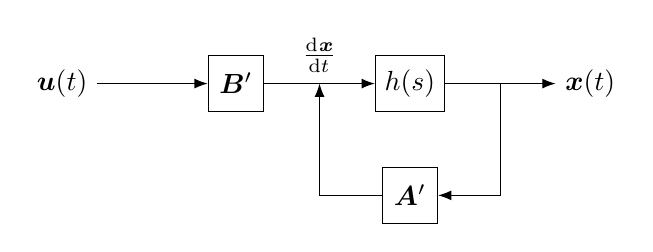
\begin{tikzpicture}[every path/.style={-Latex}, every node/.style={minimum height=20pt, minimum width=20pt}, node distance=20pt and 40pt]
    \node (u) {$\bm u(t)$};
    \node (B) [draw, right=of u] {$\bm B'$};
    \node (filt) [draw, right=of B] {$h(s)$};
    \node (x) [right=of filt] {$\bm x(t)$};
    \node (A) [draw, below=of filt] {$\bm A'$};

    \draw (u) -- (B);
    \draw (B) -- node[above] {$\od{\bm x}{t}$} (filt) coordinate[midway](Bfilt);
    \draw (filt) -- (x) coordinate[midway](filtx);
    \draw (filtx) |- (A);
    \draw (A) -| (Bfilt);
\end{tikzpicture}
\end{document}
